\setcounter{chapter}{-1}
\chapter{Review: Differential Form of the Fluid Equation}

\section{Continuity Equation}

For a \emph{system} (identifiable group of matter in space):
%
\begin{equation}
  \f{\D}{\D t}{M_{sys}} = 0
  \label{eq:mass-conversation}
\end{equation}
%
\emph{Reynolds Transport Theorem} allows us to write the mass conversation for a \emph{control volume}:
\begin{equation}
  \underbrace{\vphantom{\f{\p}{\rho}} \f{\p}{\p t} \int_{CV}{\rho \d V} }_{\substack{\text{rate of change of mass} \\ \text{in the C.V.}}}
  +
\underbrace{\vphantom{\f{\p}{\rho}}\int_{CS}{\rho \mb{U} \cdot \mb{n} \d A}}_{\substack{\text{Net rate of flow of mass} \\ \text{across C.S.}}}
  = 0
  \label{eq:reynolds-transport-theorem}
\end{equation}
%
where \(\rho\) is the density of the fluid, \(\d V\) is the infinitesimal control volume, \(\mb{U}\) is the velocity of the fluid, and \(\mb{n}\) outward unit normal vector, which is normal to the infinitesimal differential surface element \(\d A\).

To write \cref{eq:reynolds-transport-theorem} in differential form, we first consider a small fluid element of volume \(\delta V = \delta x \delta y \delta z\). We can say that \(\rho\) is uniform within a small fluid element assuming that the fluid element is small enough. Therefore, the LHS of the \cref{eq:reynolds-transport-theorem} will be
%
\begin{equation}
  \f{\p}{\p t} \int_{CV}{\rho \d V}
  = \f{\p}{\p t} \int_{CV}{\d V}
  = \left(\f{\p\rho}{\p t}\right) \left(\delta x \delta y \delta z\right)
\end{equation}
%
For the RHS of \cref{eq:reynolds-transport-theorem}, we consider the mass flux in the x-direction through faces of a cubic fluid element
%
\begin{figure}
  \begin{center}
    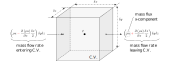
\includegraphics[width=0.95\textwidth]{differnetial-fluid-element-x}
  \end{center}
  \caption{Mass flow rate x-direction for a infinitesimal control volume.}\label{fig:fluid-element-mass-flow-rate-x-direction}
\end{figure}
%
Thus,
%
\begin{equation}
  \text{net mass outflow in x-direction} = \f{\p \left(\rho u\right)}{\p x} \delta x \delta y \delta z
  \label{eq:net-mass-outflow-x}.
\end{equation}
%
Similarly for \(y\) and \(z\) direction we will have
%
\begin{equation}
\begin{aligned}
  \text{net mass outflow in y-direction} &= \f{\p \left(\rho v\right)}{\p y} \delta y \delta x \delta z \\
  \text{net mass outflow in z-direction} &= \f{\p \left(\rho w\right)}{\p z} \delta z \delta x \delta y
\end{aligned}
  \label{eq:net-mass-outflow-y-z}.
\end{equation}

% % Figure token from Tobias Holzmann's book
% \begin{figure}[!b]
% \begin{tikzpicture}
% % Koordinatensystem
% \draw[->] (0,0) -- (7,0) node[right] {$x$} coordinate(x axis);
% \draw[->] (0,0) -- (0,5) node[above] {$z$} coordinate(z axis);
% \draw[->] (0,0) -- (1.5,1.5) node[below] {$y$} coordinate(y axis);
%
% % Quader
% \draw [fill=gray!30] (3,1) -- (5,1) -- (5,3) -- (3,3) -- (3,1) ;
%
% \draw [densely dashed] (3.5,1.5) -- (5.5,1.5);
% \draw [] (5.5,1.5) -- (5.5,3.5) -- (3.5,3.5);
% \draw [densely dashed] (3.5,3.5) -- (3.5,1.5);
%
% \draw  [densely dashed] (3,1) -- (3.5,1.5);
% \draw  [fill=gray!10] (5,1) -- (5.5,1.5) -- (5.5,3.5) -- (5,3) -- (5,1);
% \draw  [fill=gray!10] (5,3) -- (5.5,3.5) --  (3.5,3.5) -- (3,3) -- (5,3);
%
% %\draw (3,1) -- (3.5,3.5);
% %\draw (3,3) -- (3.5,1.5);
%
% % Pfeile
% % rechts nach links
% \draw [densely dotted, ->] (3,2.25) -- (3.25,2.25);
% \draw [] (1.5,2.25) -- (3,2.25);
% \draw [->] (5.25,2.25) -- (7.25,2.25);
%
% % unten nach oben
% \draw [] (4.25,0.25) -- (4.25,1);
% \draw [densely dotted, ->] (4.25,1) -- (4.25,1.25);
% \draw [->] (4.25,3.25) -- (4.25,4.25);
%
% % vorn nach hinten
% \draw [densely dotted, ->] (4.5,2.5) -- (4.75,2.75);
% \draw [->] (3.75,1.75) -- (4,2);
%
% % Punkte für Gleichungen
% \node at (2.25,2.5) {\scriptsize $ u_x|_{_x}$};
% \node at (6.5,2.5) {\scriptsize $ u_x|_{_{x+\Delta x}}$};
%
% %\node at (4.5,0.5) {\scriptsize $ u_y|_{_y}$};
% %\node at (4.5,4.2) {\scriptsize $ u_y|_{_{y+\Delta y}}$};
%
% %\node at (4.5,2.75) {\scriptsize $ u_z|_{_x}$};
% % \node at (4,1.75) {\scriptsize $ u_z|_{_{z+\Delta z}}$};
%
% % Linien für dx dy dz
% \draw [densely dashdotted] (5,1) -- (5.6,1)
%    (5.5,1.5) -- (6.1,1.5)
%    (5.5,3.5) -- (6.1, 3.5)
%    (3.5,3.5) -- (3.8,3.8)
%    (5.5,3.5) -- (5.8,3.8);
%
% \draw [<->,densely dashdotted] (5.3,1) -- (5.8,1.5);
% \node at (6,1.25) {\tiny $\Delta y$};
%
% \draw [<->,densely dashdotted] (5.8,1.5) -- (5.8,3.5);
% \node at (6.1,3.2) {\tiny $\Delta z$};
%
% \draw [<->,densely dashdotted] (3.65,3.65) -- (5.65,3.65);
% \node at (4.75,3.8) {\tiny $\Delta x$};
%
% % Volumenpunkt
% \node at (4.25,2.25) {\tiny $\bullet$};
% \node at (4.5,2.25) {\tiny d$V$};
%
%
% \node at (8.5,5) [right] {\scriptsize $ \rmm{Mass~inside~x:~} (\rho u_x)|_{_x} \Delta y \Delta z $};
% \node at (8.5,4.4) [right] {\scriptsize $ \rmm{Mass~outside~x:~} (\rho u_x)|_{_{x+\Delta x}} \Delta y \Delta z $};
%
% \node at (8.5,3.4) [right] {\scriptsize $ \rmm{Mass~inside~y:~} (\rho u_y)|_{_y} \Delta x \Delta z $};
% \node at (8.5,2.8) [right] {\scriptsize $ \rmm{Mass~outside~y:~} (\rho u_y)|_{_{y+\Delta y}} \Delta x \Delta z $};
%
% \node at (8.5,1.8) [right] {\scriptsize $ \rmm{Mass~inside~z:~} (\rho u_z)|_{_z} \Delta x \Delta y $};
% \node at (8.5,1.2) [right] {\scriptsize $ \rmm{Mass~outside~z:~} (\rho u_z)|_{_{z+\Delta z}} \Delta x \Delta y $};
%
% \end{tikzpicture}
% \caption{Mass balance in a small volume element d$V$.}
% \label{figure::massFigure}
% \end{figure}

% vim: et ts=2 sw=2
